\documentclass{beamer}

\mode<presentation>
{
   \usetheme{EEng}
%   \usetheme{Warsaw}
  \setbeamercovered{transparent}
  \setbeamercolor{background canvas}{bg=black!0}
}

\usepackage{enumerate}
\usepackage{array}
\usepackage{graphics}
\usepackage{ucs}
\usepackage[utf8x]{inputenc}
\usepackage[english]{babel}
\usepackage{amsmath, amsthm, amssymb}
\usepackage{amsmath}
\usepackage{amsfonts}
\usepackage{xcolor}
\usepackage{pgf}
\usepackage{hyperref}
\usepackage{url}
\usepackage{multicol}   % add-on
\usepackage{boxedminipage} 
\usepackage{indentfirst}   % add-on
\usepackage{float}
\usepackage[all]{xypic}
\usepackage{listings}
\usepackage{verbatim}
\usepackage{boxedminipage}

% % % inicio do listings e ref
\definecolor{darkblue}{rgb}{0,0,0.6}
\definecolor{gray_ulisses}{gray}{0.55}
\definecolor{castanho_ulisses}{rgb}{0.71,0.33,0.14}
\definecolor{preto_ulisses}{rgb}{0.41,0.20,0.04}
\definecolor{green_ulises}{rgb}{0.2,0.75,0}

\hypersetup{
	a4paper,
	pdftex,
	bookmarks,
	colorlinks,
    citecolor=darkblue,
    linkcolor=darkblue,
    urlcolor=darkblue,
    filecolor=darkblue
}

\lstdefinelanguage{Terminall} {
       basicstyle=\scriptsize\ttfamily,
       breaklines=true,
       breakautoindent=false,
       showstringspaces=false
}
\lstdefinelanguage{Terminal} {
       basicstyle=\tiny\ttfamily,
       breaklines=true,
       breakautoindent=false,
       showstringspaces=false
}
\definecolor{gray_ulisses}{gray}{0.55}
\definecolor{castanho_ulisses}{rgb}{0.71,0.33,0.14}
\definecolor{preto_ulisses}{rgb}{0.41,0.20,0.04}
\definecolor{green_ulises}{rgb}{0.2,0.75,0}

\lstdefinelanguage{HaskellUlisses}
{
        basicstyle=\ttfamily\scriptsize,
        %backgroundcolor=\color{yellow},
        %frameshape={RYRYNYYYY}{yny}{yny}{RYRYNYYYY}, %contornos... muito nice...
        sensitive=true,
        morecomment=[l][\color{gray_ulisses}\ttfamily\tiny]{--},
        morecomment=[s][\color{gray_ulisses}\ttfamily\tiny]{\{-}{-\}},
        morestring=[b]",
        stringstyle=\color{red},
        showstringspaces=false,
%       numbers=left,
%       firstnumber=\thelstnumber,
        numberstyle=\tiny,
        numberblanklines=true,
        showspaces=false,
        breaklines=true,
        showtabs=false,
%       xleftmargin=15pt,
%       xrightmargin=-20pt,
        emph=
        {[1]
                FilePath,IOError,abs,acos,acosh,all,and,any,appendFile,approxRational,asTypeOf,asin,
                asinh,atan,atan2,atanh,basicIORun,break,catch,ceiling,chr,compare,concat,concatMap,
                const,cos,cosh,curry,cycle,decodeFloat,denominator,digitToInt,div,divMod,drop,
                dropWhile,either,elem,encodeFloat,enumFrom,enumFromThen,enumFromThenTo,enumFromTo,
                error,even,exp,exponent,fail,filter,flip,floatDigits,floatRadix,floatRange,floor,
                fmap,foldl,foldl1,foldr,foldr1,fromDouble,fromEnum,fromInt,fromInteger,fromIntegral,
                fromRational,fst,gcd,getChar,getContents,getLine,head,id,inRange,index,init,intToDigit,
                interact,ioError,isAlpha,isAlphaNum,isAscii,isControl,isDenormalized,isDigit,isHexDigit,
                isIEEE,isInfinite,isLower,isNaN,isNegativeZero,isOctDigit,isPrint,isSpace,isUpper,iterate,
                last,lcm,length,lex,lexDigits,lexLitChar,lines,log,logBase,lookup,map,mapM,mapM_,max,
                maxBound,maximum,maybe,min,minBound,minimum,mod,negate,not,notElem,null,numerator,odd,
                or,ord,otherwise,pi,pred,primExitWith,print,product,properFraction,putChar,putStr,putStrLn,quot,
                quotRem,range,rangeSize,read,readDec,readFile,readFloat,readHex,readIO,readInt,readList,readLitChar,
                readLn,readOct,readParen,readSigned,reads,readsPrec,realToFrac,recip,rem,repeat,replicate,return,
                reverse,round,scaleFloat,scanl,scanl1,scanr,scanr1,seq,sequence,sequence_,show,showChar,showInt,
                showList,showLitChar,showParen,showSigned,showString,shows,showsPrec,significand,signum,sin,
                sinh,snd,span,splitAt,sqrt,subtract,succ,sum,tail,take,takeWhile,tan,tanh,threadToIOResult,toEnum,
                toInt,toInteger,toLower,toRational,toUpper,truncate,uncurry,undefined,unlines,until,unwords,unzip,
                unzip3,userError,words,writeFile,zip,zip3,zipWith,zipWith3,listArray,doParse
        },
        emphstyle={[1]\color{blue}},
        emph=
        {[2]
                Bool,Char,Double,Either,Float,IO,Integer,Int,Maybe,Ordering,Rational,Ratio,ReadS,ShowS,String,
                Word8,InPacket
        },
        emphstyle={[2]\color{castanho_ulisses}},
        emph=
        {[3]
                case,class,data,deriving,do,else,if,import,in,infixl,infixr,instance,let,
                module,of,primitive,then,type,where
        },
        emphstyle={[3]\color{preto_ulisses}\textbf},
        emph=
        {[4]
                quot,rem,div,mod,elem,notElem,seq
        },
        emphstyle={[4]\color{castanho_ulisses}\textbf},
        emph=
        {[5]
                EQ,False,GT,Just,LT,Left,Nothing,Right,True,Show,Eq,Ord,Num
        },
        emphstyle={[5]\color{preto_ulisses}\textbf}
}
% % % fim do listings e ref

% % % inicio da definicao de comandos

% % % fim da definicao de comandos

\title{SOPAS - Submissão Online Para Análise de Software}
\author{José Pedro Silva \and
Pedro Faria \and
Ulisses Costa
}

\date{\today}
\institute{Engenharia de Linguagens\\
Projecto integrado
}

\AtBeginSubsection[] {
  \begin{frame}<beamer>
    \frametitle{Index}
    \scriptsize{\tableofcontents[currentsection,currentsubsection]}
  \end{frame}
}

\AtBeginSection[] {
  \begin{frame}<beamer>
    \frametitle{Index}
    \scriptsize{\tableofcontents[currentsection]}
  \end{frame}
}
\begin{document}
\begin{frame}
   \titlepage
\end{frame}

\section{Até agora}
\begin{frame} \frametitle{Até agora:}
Concretizado até ao ínicio da segunda fase:
\begin{itemize}
\item Descrição do sistema {\color{green}$\checkmark$}
\item Modelação formal e informal do problema {\color{green}$\checkmark$}
\item Modelo de dados {\color{green}$\checkmark$}
\item Ínicio da implementação e respectivo tool demo {\color{green}$\checkmark$}
\end{itemize}
\end{frame}

\section{Objectivos}
\pgfdeclareimage[width=.8\textwidth]{topo}{images/topo}

\begin{frame} \frametitle{Motivação e Objectivos}
Objectivos para segunda fase:
\begin{itemize}
\item Terminar a aplicação web \\
- compilar e executar o código fonte submetido\\
- guardar e apresentar resultados\\
\item Investigação das métricas existentes
\item Scripts auxiliares
\item Exploração de um frontend
\end{itemize}
\end{frame}

\section{Aplicação Web}

\subsection{Implementação: até à segunda fase}
\begin{frame} \frametitle{Implementação: até à segunda fase}
Já implementado para o último checkpoint:
\begin{itemize}
\item Criação de contas de utilizador (grupo)
\item Associação de concorrentes a determinado grupo
\item Criação de concursos
\item Criação de enunciados (através da interface web ou submetendo em formato xml)
\item Inserção de baterias de teste para os enunciados
\item Submissão de programas para avaliação
\end{itemize}
\end{frame}

\subsection{Implementação: linguagens de programação}
\begin{frame} \frametitle{Implementação: linguagens de programação}
Configuração de linguagens de programação:
\begin{itemize}
\item Estando a linguagem correctamente configurada no servidor, é 
simples preparar o sistema de submissão para avaliar código submetido nessa linguagem
\item Para isso basta inserir o comando usado para compilar e para executar, que por exemplo, em C seria:\\
String compilação: \textit{gcc -O2 -Wall \#\{file\}}\\
String de execução default: \textit{./a.out}\\
String de execução para makefile: \textit{./\#\{file\}}
\end{itemize}
\end{frame}

\subsection{Implementação: Compilação}
\begin{frame} \frametitle{Implementação: Compilação}
\begin{itemize}
\item Caso seja necessário compilar o código fonte submetido, é usada a string de compilação definida
aquando da configuração da linguagem
\item Se for submetido um ficheiro comprimido que inclua um makefile, é executado o comando \textit{make} e, 
o nome do executável criado é obtido a partir de um script perl
\end{itemize}
\end{frame}

\subsection{Implementação: Execução}
\begin{frame} \frametitle{Implementação: Execução}
\begin{itemize}
\item Para executar o programa para os diferentes inputs, é usada a string de execução simples (no caso de ser submetido
apenas um ficheiro) ou a string de execução para makefile (no caso de ser submetido um makefile)
\item Para cada input o comando é corrido uma vez
\item O output é capturado e comparado com o esperado
\item É guardada a percentagem de testes no qual o código submetido passou
\end{itemize}
\end{frame}

\begin{frame} \frametitle{Implementação: Apresentação de resultados}
\begin{itemize}
\item A qualquer altura o utilizador pode consultar os resultados das últimas submissões (suas ou dos restantes 
participantes)
\item Pode também consultar os seus melhores resultados, para cada enunciado

\begin{figure}[H]
\begin{center}
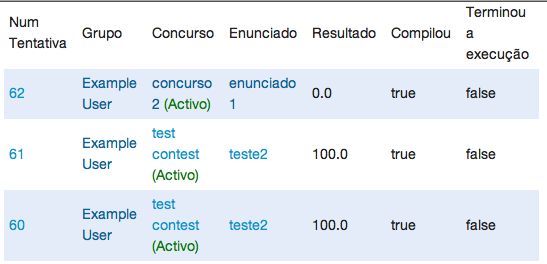
\includegraphics[width=0.75\textwidth]{imagens/tentativas}
%\caption{Página de registo}\label{img:signup}
\end{center}
\end{figure} 

\end{itemize}
\end{frame}

\section{Scripts Auxiliares}
\begin{frame} \frametitle{Scripts auxiliares}
\begin{itemize} 
\item Script (em Perl) para obter o nome do executável gerado pelo makefile (para C)
\item Script (em Perl) que gera estatísticas relativamente à quantidade de ficheiros submetidos para cada linguagem de programação
\end{itemize}
\end{frame}

\begin{frame} \frametitle{Script makefile.pl}
\begin{itemize} 
\item Utiliza o módulo perl \textit{Makefile::Parser} para fazer parse do makefile, e obter o nome do executável gerado
\item No caso de não ser definido um nome para o output, retorna \textit{a.out}
\item TODO: Suportar mais linguagens par além do C.
\end{itemize}
\end{frame}

\begin{frame} \frametitle{Script count.pl}
\begin{itemize} 
\item Dada uma pasta, explora recursivamente os seus directórios, e extraí várias estatisticas relativas á quantidade de número de linhas
  \begin{itemize}
    \item Número de linhas de código por linguagem
    \item Número de linhas comentadas por linguagem
	\item Rácio entre linhas de código e número de ficheiros para cada linguagem
	\item Percentagem de linguagem mais usadas no projecto
	\item ...
  \end{itemize}
\item Utiliza o módulo perl \textit{GD} para gerar gráficos
\end{itemize}
\end{frame}

\section{Frontend}
\begin{frame} \frametitle{Language.C}
\end{frame}

\section{Terminal Interface - Powered by Perl}
\begin{frame} \frametitle{Terminal Interface}
\begin{itemize}
 \item Criado para facilitar a manutenção e o acesso à base de dados.
 \item Interface utilizada apenas pelos \textbf{administradores} do sistema.
\end{itemize}
\end{frame}

\begin{frame} \frametitle{Terminal Interface - Perl}
Escolheu-se esta linguagem devido:
\begin{itemize}
 \item Rápida implementação
 \item Vasta diversificação de módulos
\end{itemize}
Desses módulos, usa-se e pretende-se usar:
\begin{itemize}
 \item \textbf{DBIx::Class}
 \item \textbf{Term::Readline}
 \item \textbf{Digest::SHA2}
 \item \textbf{XML::DT}
\end{itemize}
\end{frame}

\begin{frame} \frametitle{Estado actual}
 Exemplo actual da interface:
\begin{figure}[H]
\begin{center}
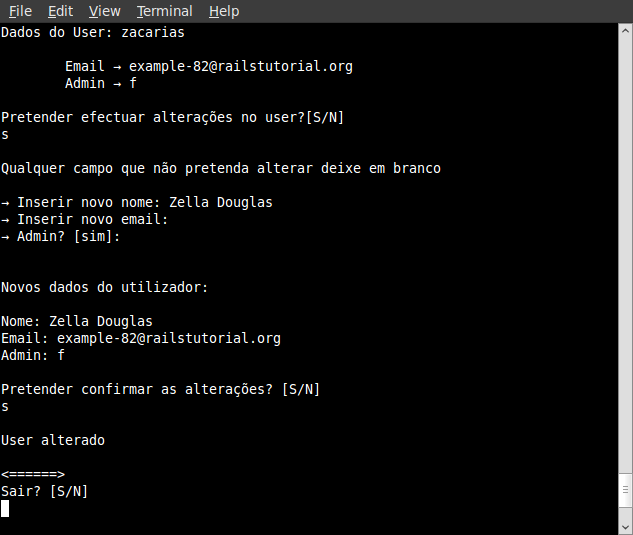
\includegraphics[width=0.65\textwidth]{imagens/zacarias}
%\caption{Página de registo}\label{img:signup}
\end{center}
\end{figure} 
\end{frame}


\section{Conclusão e trabalho futuro}
\begin{frame} \frametitle{Conclusão e trabalho futuro}
\begin{itemize}
\item Implementar várias métricas para C com o FrontEnd
\item Tornar a interface utilizador mais intuitiva e mais agradável de utilizar
\end{itemize}
\end{frame}


\section*{Perguntas}
\begin{frame} \frametitle{Perguntas}
\begin{center}\huge{?}\end{center}
\end{frame}

\end{document}
